\chapter{Construction dynamique d'une relation interpersonnelle de dominance}
\label{chap:Tom}
\begingroup
\parindent=0em
\etocsettocstyle{\rule{\linewidth}{\tocrulewidth}\vskip0.5\baselineskip}{\rule{\linewidth}{\tocrulewidth}}
\emph{\textbf{Sommaire}}
\localtableofcontents 
\clearpage
\endgroup

Afin d'étudier l'impact d'une relation interpersonnelle de dominance sur les stratégies de négociations entre un agent conversationnel et un humain, l'agent doit être en mesure de simuler une relation de dominance entre lui et l'utilisateur humain. Pour ce faire, l'agent doit détecter les comportements de dominance de son interlocuteur afin d'adapter son comportement en complémentarité. Nous proposons dans ce chapitre un algorithme pour simuler les comportements de dominance de l'interlocuteur. 

A partir de notre modèle de négociation collaborative présenté dans la chapitre \ref{chap:dec}, nous proposons une extension qui permet à l'agent de raisonner sur les comportements de dominance de son interlocuteur, et d'automatiquement adapter ses comportements à ceux perçus chez son interlocuteur dans le but de créer une relation complémentaire de dominance.

Dans la section 1, nous présentons brièvement le modèle théorique de la théorie de l'esprit sur lequel se base notre approche pour raisonner sur les comportements de l'interlocuteur. Par la suite, nous présentons une première solution naïve et nous discuterons ses limites. Ensuite, dans la section 3, nous détaillons notre solution et nous présentons dans la section 4 son évaluation.  




\section{Croyances sur l'autre: Théorie de l'esprit}
Notre but est de proposer un modèle de négociation collaborative capable de simuler une relation interpersonnelle de dominance. La relation de dominance étant complémentaire, l'agent doit être capable de prédire les comportements de dominance de son interlocuteur afin d'adopter un comportement complémentaire comme présenté dans la figure \ref{fig:schema-general}. 
Ce processus d'attribution d'état mentaux sur les comportements de l'interlocuteur est appelé théorie de l'esprit ou \emph{Theory Of Mind} (ToM). Ce dernier est un processus cognitif permettant à un individu un individu d'attribuer des états mentaux tels que des croyances, intentions et désirs à autrui afin de mieux comprendre, expliquer, prédire ou manipuler les comportements de ses interlocuteurs \cite{harbers2012modeling}. Il a été démontré que la ToM est un concept crucial dans la compréhension des interactions humaines \cite{whiten1991natural,byom2013theory}. Pour cette raison, un nombre importants de travaux ont étudié les mécanismes de la ToM. Cependant, un débat subsiste sur la nature des mécanismes de théorie de l’esprit partagés entre deux approches: une approche \textit{theory-theory}  \emph{(TT)} et une approche \textit{simulation theory} \emph{(ST)} \cite{harbers2012modeling,shanton2010simulation}.

Les défenseurs de l'approche \textit{theory-theory} (TT) postulent que la ToM s’appuie sur une représentation implicite du raisonnement de l'autre construite à partir d'un ensemble de concepts tels que les désirs, les croyances ou les plans de l'autre \cite{harbers2012modeling}. En effet, cette théorie se base sur une représentation basique de l'environnement \emph{"folk theory"}. A partir de comportements observés chez l'autre, l'individu fait des inférences théoriques sur ses états mentaux \cite{shanton2010simulation}.

En revanche, les partisans de simulation théorie(ST) suggèrent que les humains ont la capacité de se projeter dans la perspective d'une autre personne \cite{shanton2010simulation}.
Par conséquent, ils peuvent simuler l'activité mentale d'autrui avec leurs propres capacités de raisonnement pratiques. Cela leurs permet d'imiter l'état mental de leurs partenaire interactionnel \cite{harbers2009modeling}.
Par ailleurs, cette approche stipule qu'il n'est pas pas nécessaire d'être capable d'introspection complète de l'autre pour simuler ses processus mentaux. En d'autres mots, il n'est pas nécessaire de catégoriser toutes les croyances et les désirs attribués à cette personne pour pouvoir simuler son état mental \cite{harbers2012modeling}.

Enfin, les partisans de la \emph{ST} ajoutent que la simulation est plus efficace que l'acquisition d'une théorie complète. Pour ces raisons, certains partisans de la théorie-théorie admettent qu'au moins une certaine forme de simulation doit avoir lieu lorsque les gens raisonnent au sujet d'autrui, et incorporent des aspects de simulation dans une approche théorie-théorie \cite{harbers2012modeling}.

Dans le contexte de cette thèse, nous utiliserons l'approche de \emph{simulation théorie (ST)} qui permet d'utiliser le modèle de décision de l'agent pour raisonner sur les comportements de dominance de l'interlocuteur. 

Dans la suite de ce chapitre, nous présentons notre algorithme pour simuler le comportement de l'interlocuteur.


\section{Approche naïve}
L'agent dispose d'un modèle de négociation dont les stratégies décisionnels reposent sur les comportements de dominance. Ce modèle fut validé durant une interaction agent/agent et agent/humain. Par conséquent, afin de modéliser le fonctionnement de l'état mental de l'interlocuteur, nous proposons une solution basé sur la \emph{ST}, pour laquelle nous adaptons le modèle décisionnel de l'agent pour qu'il raisonne sur les comportements de son interlocuteur. 

\begin{sidewaysfigure}
	\centering
	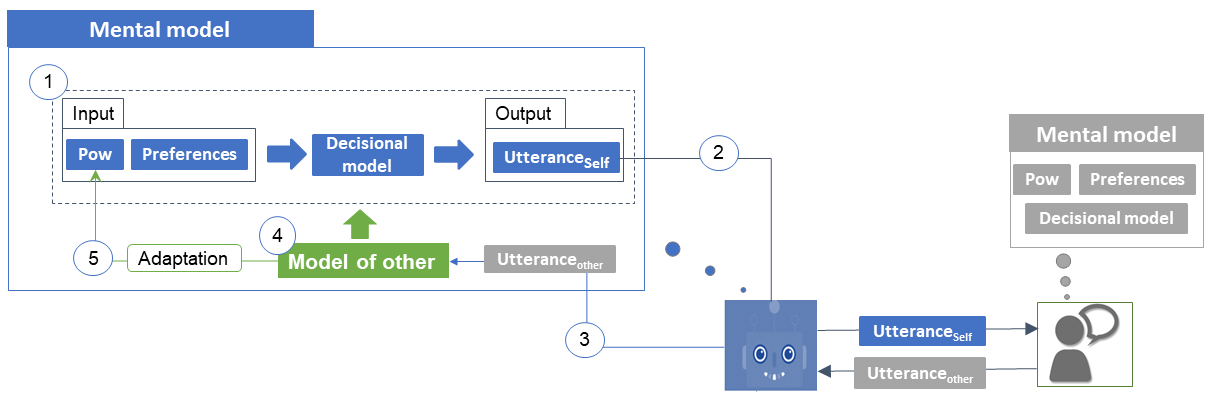
\includegraphics[width=\linewidth, height=0.35\textheight]{Figures/chap5/model/general.png}
	\caption{Modèle de négociation collaborative avec un modèle de l'interlocuteur. Processus de décision étape par étape} 
	\label{fig:schema-general}
\end{sidewaysfigure}
	



Le modèle décisionnel de l'agent est régi par son état mental: ses préférences ainsi que sa position dans le spectre de dominance. Une proposition naïve pour adapter ce modèle afin qu'il raisonne sur les comportements de l'interlocuteur consisterait à formuler des hypothèses sur l'état mental de l'interlocuteur. 

En effet, pour chaque hypothèse sur l'état mental, l'agent appelle son modèle décisionnel  pour simuler les réponses possibles de son interlocuteur dans le contexte courent de la négociation. Ensuite, l'agent compare les réponses produites par la simulation avec l'acte de dialogue de l'interlocuteur $utterance_{other}$ produite dans l'étape 3 (voir la figure \ref{fig:schema-general}). 
La dernière étape consiste à mettre à jours les hypothèses jusqu'à converger à une valeur de dominance précise. 

Toutefois, cette approche repose sur quelques hypothèses fortes. Tout d'abord, nous supposons que le modèle de décision est une représentation précise du processus décisionnel de l'utilisateur. Il n'y a aucun moyen de garantir cette hypothèse. Cependant, dans le chapitre \ref{chap:dec}, nous avons montré que les comportements de dominance exprimés par les agents, générés à partir de ce modèle de décision, sont correctement perçus par les utilisateurs humains. 
De plus, nous partons du principe que notre système soit capable de générer toutes les hypothèses sur l'état mental de l'interlocuteur pour n'importe quel domaine de négociation. C'est à dire, pour chaque hypothèse formulée sur une valeur de dominance, générer l'ensemble de modèles de préférences $\prec_i$ pour chaque critère. Ce processus peut être complexe en raison d'une infinité de possibilités. Pour cette raison, nous considérons que dix valeurs possibles pour les valeurs de dominance. 

	\subsection{Algorithme de ToM}
Sur la base de ces hypothèses, nous présentons l'algorithme général du modèle d'état mental de l'interlocuteur illustré dans la figure \ref{fig:schema-general} comme suit:

\begin{enumerate}
	\item Construire l'ensemble $H_{dom}$ des la valeur de dominance potentielles de l'interlocuteur : $h\in H_{dom}$ représente la possibilité que la valeur $h$ soit la valeur réelle de dominance $dom_{other}=h$. Nous considérons 9 valeurs de dominance: $H_{dom}=\{0.1, 0.2, \ldots, 0.9\}$.
	
	\item Pour chaque valeur $h$, construire l'ensemble des préférences possibles $Prec_h$: les éléments $p\in Prec_h$ sont des préférences, c'est à dire des ordres sur l'ensemble des éléments de $\mathcal{C}$.
	
	\item Après chaque acte de dialogue reçu $u$ de la part de l'interlocuteur, supprimer tout les éléments de $Prec_h$ qui ne sont pas compatibles avec $u$. Concrètement, si la condition d'applicabilité de $u$ n'est pas satisfaite dans $p \in Prec_h$, alors $p$ doit être retirée des états mentaux candidats.
	\item Pour chaque état mental potentiel: pour chaque $h$ et pour chaque $p \in  Prec_h$,  calculer l'acte de dialogue obtenu à l'issue du processus décisionnel (suivant l'approche de la \emph{simulation-theory}).s
	\item Calculer le $score(h)$ comme le nombre d'hypothèses restantes $|Prec_h|$ générant le même acte de dialogue que celui produit par l'interlocuteur $Utterance_{other}$. 
	\item 	La valeur $h \in H_{dom}$ avec le score le plus élevé est est considéré comme la plus proche de l'état mental de l'interlocuteur.
	$$dom_{other} = \operatorname*{arg\,max}_{h} (score(h))$$
\end{enumerate}

	\begin{figure*}
		\centering
		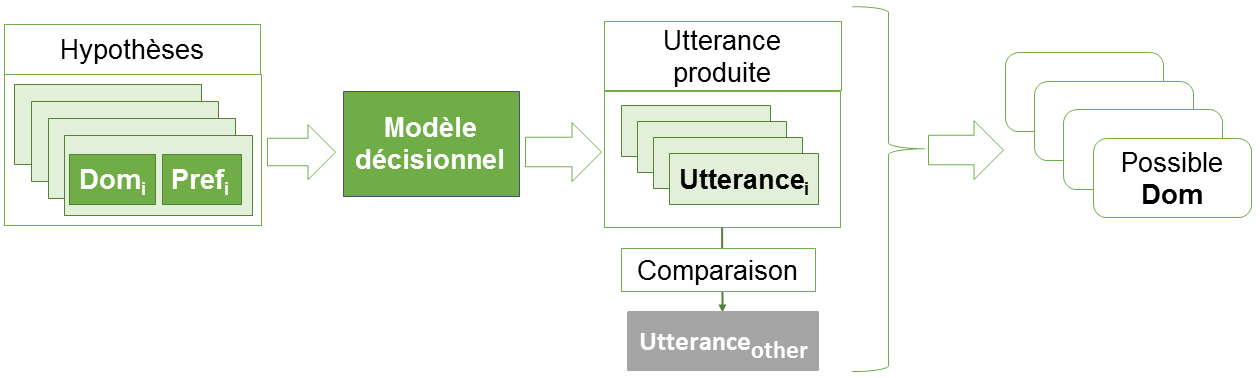
\includegraphics[width=\linewidth]{Figures/chap5/model/tom_select.PNG}
		\caption{Modèle de la ToM pour évaluer les hypothèses sur le niveau de dominance d'un interlocuteur à partir de son acte de dialogue} 
		\label{fig:tom}
	\end{figure*} 
	
\subsection{Limites de l'approche naïve: Représentation des préférences}

L'approche proposée repose sur la capacité de notre système a générer toutes les états mentaux possibles et à les réviser à chaque tour de parole en temps réel. La génération de toutes les relations de préférences est coûteuse. En effet, afin de générer l'ensemble des préférences pour chaque valeur de dominance possible, nous devons considérer tout les ordres partiels $\prec_i$ pour chaque critère $C_i$. 

Nous pouvons calculer la taille de l'ensemble des relations de préférences binaires en fonction du nombre de valeurs défini dans le domaine de négociation. Ainsi, pour un critère $C_i$, l'ensemble ordre partiel possibles est  $(|C_i|+1)! $. Par conséquent, pour un sujet de négociation avec $n$ critères , il y a $\prod_{i=1}^n (|C_i|+1)!$ ensembles de préférences possibles.


Si nous considérons un exemple raisonnable, avec 5 critères. Pour chaque critère, nous considérons environ 4 à 10 valeurs possibles pour chaque domaine de critère. L'ensemble des préférences possibles pour le modèle de l'interlocuteur est compris entre $ 24.10 ^ 9 $ et $ 10 ^ {38} $ ensembles de préférences possibles.
Nous pouvons facilement conclure qu'il n'est pas raisonnable de considérer toutes ces hypothèses, une à une, à chaque étape du dialogue.

Par ailleurs, le but de notre modèle est de reconstituer les comportements de dominance de l'interlocuteur et non pas ses préférences. Pour cela, il faut avoir un minimum de connaissance sur les préférences de l'interlocuteur. Cependant, modéliser l'ensemble des relations de préférences possibles ne semble pas réaliste et probablement pas utile.

Cette limite nous a poussé à analyser plus en détails l'utilisation des préférences durant le processus décisionnel. Comme nous l'avions présenté dans le chapitre \ref{chap:dec}, les préférences sont requises pour calculer la satisfiabilité des valeurs. Cette valeur de satisfiabilité est essentielle durant le processus décisionnel. Pour cause, l'agent l'utilise pour calculer l'ensemble de valeurs satisfiables $S$ ainsi que les valeurs acceptables $Ac(t)$.

La satisfiabilité est calculée à partir du nombre de prédécesseurs dans l'ordre des relations binaires de préférences, et l'acceptabilité à partir des valeurs de satisfiabilité. Nous proposons, donc, un modèle qui reconstitue le calcul de ses deux valeurs afin de limiter l'explosion combinatoire causé par les relations de préférences. 

\subsubsection{Relation d'ordre sur les préférences}
	Les relations d'ordre sur les préférences peuvent être totales ou partielles. En effet, en fonction du domaine de négociation, un agent peut avoir un ordre de préférence stricte où chaque valeur est comparable à toutes les autres. Au contraire, il se peut dans un autre contexte, qu'un agent n'est pas un ordre total de préférences, c'est à dire, que l'agent peut n'avoir aucune préférence entre deux valeurs $a$ et $b$ du domaine. Pour autant, nous pouvons générer un ensemble d'ordre totaux à partir d'un ordre partiel. Par exemple, nous pouvons suppose que l'agent $a \prec b$ ou bien au contraire $b \prec a$. Cette supposition n'affecte pas énormément le processus décisionnel de l'agent. 
	
	Néanmoins, un ordre total de préférence facilite la simulation des comportement d'autrui. En effet, supposons un \textit{ordre total} de préférences $\prec_j$, dans lequel toutes les valeurs sont comparables, donc nous avons $|\prec_j| -1$ relations binaires de préférences. Indépendamment des valeurs elles-mêmes, en connaissant seulement le nombre de valeurs, nous somme capables de calculer la satisfiabilité de chaque valeur à partir de son rang dans l'ordre de préférences.

	Par exemple, considérons le critère $cuisine$ composé de quatre valeurs $\{jap,it,fr,ch\}$ sur lequel est défini un ensemble de préférences d'ordre total $\prec_{cuisine} = \{jap$$\prec$ $fr, fr$$\prec$$ ch, ch$$\prec$$it\}$, la satisfiabilité des valeurs est présenté dans la table \ref{tab:ex2_sat}. Considérons maintenant, un second ordre total de préférences $\prec'_{cuisine} = \{it$$\prec$ $jap, jap$$\prec$$ fr, fr$$\prec$$ch\}$, nous remarquons que les valeurs de satisfiabilité sont les mêmes que celles pour le modèle $\prec_{cuisine}$ illustré dans la table \ref{tab:ex2_sat}. 


	\begin{table} [h]
		\centering
		\caption{Valeurs de satisfiabilité des éléments du critères $cuisine$.}
		\begin{tabular}{ |c|c|c|c|c| }
			\hline
			value & $jap$ & $fr$ & $ch$ & $it$ \\	
			\hline
			sat(value) $\prec_{cuisine}$ & 0 & 0.33 & 0.66 & 1 \\
			\hline
			sat(value) $\prec'_{cuisine}$ & 0.33 & 0.66 & 1 & 0 \\
			\hline
		\end{tabular}
		
		\label{tab:ex2_sat}
		
	\end{table}
	
	Par conséquent, dans un \emph{ordre total} de préférence pour un critère donné, seul le nombre de valeurs est nécessaire pour définir leur rang dans l'ordre de préférences et ainsi calculer leur satisfiabilités comme il est présenté dans la table \ref{tab:poss}. 


	\begin{table}[h]
		\caption{Satisfiabilité déduite à partir d'un ensemble de quatre éléments.}
		\label{tab:poss}
		\centering
		
		\begin{tabular}{ |c|c|c|c|c| }
			\hline				
			rang(valeur) & 1 & 2 & 3 & 4 \\
			\hline
			Nb prédécesseurs & 3 & 2 & 1& 0 \\
			\hline
			$sat(valeur)$ & 0 & 0.33 & 0.66 &1 \\
			\hline
		\end{tabular}
	\end{table}
	
	A partir des valeurs de satisfiabilité d'un critère donné, et la valeur de dominance de l'agent $dom$, nous pouvons déduire le nombre de valeurs satisfiables, sans pour autant connaître les relations binaires de préférences. 
	
	Par exemple, pour le critère $cuisine$ présenté plus haut, associé à une valeur de dominance $dom= 0.6$
	nous pouvons calculer la taille de l'ensemble $S$ pour n'importe quel modèle de préférences d'ordre total. En effet, à partir des valeurs de satisfiabilité présentées dans la table \ref{tab:poss},  nous pouvons conclure que le nombre de valeurs satisfiables de l'agent est toujours $|S| = 2$.
	\subsubsection{Représentation partielle des préférences}
	Dans le but de réduire le coût généré par la simulation des relations de préférences possibles de l'interlocuteur, nous proposons une modélisation partielle de son état mental en calculant uniquement le nombre de valeurs satisfiables $|S|$ pour chaque critère. Concrètement, considérons un critère avec $n$ valeurs défini avec un ordre total de préférences. Pour une valeur de dominance $dom$ donnée, nous pouvons calculer la taille de l'ensemble $S$ que nous notons $s$. 
	
	Par conséquent, nous générons uniquement des hypothèses sur les valeurs $v \in S$ qui seront satisfiables pour l'agent. Ainsi,
	la génération des hypothèses concernant les valeurs de l'ensemble $S$ sont au nombre de  $\binom{n}{s}$ possibilités. 
	
	Par exemple, pour le critère $cuisine$ et une valeur de dominance $dom =0.6$, nous avons déduit la taille de l'ensemble $S$ à $s=2$. Donc, la génération des hypothèses sur les valeurs satisfiables possible est au nombres de 6 modèles comme il est présenté dans la table \ref{tab:sat_poss}.
	\begin{table}[h]
		\centering
		\caption{L'ensembles des $S$ possibles pour le critère $cuisine$, avec $dom=0.6$}
		\label{tab:sat_poss}
	
		\begin{tabular}{|c|c|c|}%|p{1.9cm}|p{2.25cm}|p{2cm}|p{2.25cm}|p{2cm}|p{2.25cm}| }
			\hline
			$S_1=(it,fr)$& $S_2=(it,jap)$ & $S_3=(it,ch)$\\
			\hline
			$S_4=(fr,jap)$ & $S_5=(fr,ch)$ & $S_6=(jap,ch)$ \\
			\hline
		\end{tabular}
	\end{table}
	
	Cette représentation partielle des préférences à l'avantage de réduire l'ensemble des hypothèses en comparaison avec l'approche naïve qui nécessitait une représentation complète des préférences. En effet, Si l'on considère le même exemple, avec 5 critères et 10 valeurs par critère, le nombre maximum d'hypothèses à considérer pour une valeur de dominance donnée est de $ \binom {10} {5} = 252 $ (cette valeur est maximale pour $ dom = 0,5 $).
	
	Cependant, simuler le comportement de l'interlocuteur avec une connaissance incomplète de son état mental a deux conséquences.
	Premièrement, il faut réviser  le modèle décisionnel de l'agent pour qu'il puisse gérer une représentation partielle des valeurs satisfiables $S$ et les valeurs acceptables $Ac(t)$. Deuxièmement, cette adaptation pourrait affecter la précision des prédictions des comportements de dominance de l'interlocuteur.
	
	Dans la suite de ce chapitre, nous présentons notre modèle de raisonnement avec connaissance partielle ainsi que son évaluation. 
	
	

\section{Modèle de raisonnement avec représentation partielle de l'état mental}
La représentation partielle de l'état mentale repose sur une hypothèse forte. En effet, nous faisons l'hypothèse que l'interlocuteur a un \textit{ordre total} sur ses préférences. Par conséquent, pour chaque hypothèse $h\in H_{dom} $ formulée sur la valeur de dominance, et pour chaque critère, nous générons le nombre de valeurs satisfiables $s$ qui nous permet par la suite de calculer les hypothèses possibles sur les valeurs satisfiables $v\in S$ que nous notons $M_h(dom)$. Nous présentons dans la table ~\ref{tab:hypo} un exemple de génération des hypothèses sur les valeurs satisfiables calculées pour le critère $cuisine$. 

A partir de de l'acte de dialogue reçu par l'interlocuteur $utterance_{other}$, l'agent doit simuler le comportement de l'interlocuteur pour chaque hypothèse $h_i \in H_{dom}$ et ce, pour chaque hypothèse sur les préférences partielles. Pour ce faire, nous présentons l'adaptation du modèle décisionnel de l'agent pour gérer l'incertitude sur les préférences de l'interlocuteur. 
	\subsection{Principe général}
	La proposition générale de ce modèle consiste à réviser les hypothèses sur l'état mental de l'interlocuteur après chaque réception d'un nouvel acte dialogique de l'interlocuteur $utterance_{other}$. Suivant le type d'acte de dialogue reçu, l'agent calcule pour chaque hypothèse, un score $score(h_i,t)$ représentant l'exactitude de cette hypothèse à représenter le comportement exprimé par l'interlocuteur. Ensuite, l'agent associe la valeur de dominance de l'interlocuteur à l'hypothèse qui a obtenu le meilleur score:
	\begin{equation}
	dom_{other} = \operatorname*{arg\,max}_{h_i \in H_{dom}} (score(h_i,t))
	\end{equation}
	
	Nous détaillons le processus de simulation en fonction du type d'acte de dialogue reçu. En effet, pour chaque acte, l'agent va faire appel à un module de décision qui reflète un principe de dominance. Par conséquent, nous présentons l'adaptation de chaque module décisionnel pour simuler le comportement de l'interlocuteur avec des connaissances partielles.
	\begin{table}[h]
		\centering
		\caption{Hypothèses sur les valeurs satisfiables du critère $cuisine$}
		\begin{tabular}{  >{\centering\arraybackslash}m{2cm}  >{\centering\arraybackslash}m{1.5cm}  >{\centering\arraybackslash}m{6.5cm}}
			\hline
			\hline
			& \multicolumn{2}{c}{Hypothèses}  \\
			\hline
			\hline
			Hypothèse & $h_i(dom)$ & Hypothèses des valeurs satisfiables $ M_h(h_i)$\\
			\hline
			H1&0.3&$\{(fr,it,jap)\}$, $\{(fr,it,ch)\}$, $\{(fr,jap,ch)\}$, $\{(it,jap,ch)\}$ \\
			\hline
			H2&0.4&$\{(fr,it)\}$, $\{(fr,jap)\}$, $\{(fr,ch)\}$, $\{(it,jap)\}$, $\{(it,ch)\}$, $\{(jap,ch)\}$ \\
			\hline
			H3&0.5&$\{(fr,it)\}$, $\{(fr,jap)\}$, $\{(fr,ch)\}$, $\{(it,jap)\}$, $\{(it,ch)\}$, $\{(jap,ch)\}$\\
			\hline
			H4&0.6&$\{(fr,it)\}$, $\{(fr,jap)\}$, $\{(fr,ch)\}$, $\{(it,jap)\}$, $\{(it,ch)\}$, $\{(jap,ch)\}$ \\
			\hline
			H5&0.7&$\{(fr)\}, \{(it)\}, \{(jap)\}, \{(ch)\}$\\
			\hline
			H6&0.8&$\{(fr)\}, \{(it)\}, \{(jap)\}, \{(ch)\}$ \\
			\hline
			
			H7&0.9&$\{(fr)\}, \{(it)\}, \{(jap)\}, \{(ch)\}$ \\
			\hline
			\hline
		\end{tabular}		
		\label{tab:hypo}
	\end{table} 

	\subsection{Contrôle de la négociation}	
	
	Nous avons présenté dans la section \ref{chp4:controle}, l'algorithme  choisi une stratégie d'acte de dialogue en fonction de la valeur de dominance. Nous avons démontré qu'un agent avec une valeur haute dans le spectre de dominance utilisait plus fréquemment des \emph{actes de négociations}. A l'opposé, une expression fréquente des \emph{actes informatif} traduisait un comportement de soumission (faible dominance). 
	
	Nous notons \textit{history}, la liste des actes de dialogue énoncés par l'interlocuteur tout au long de la négociation. L'estimation de la dominance de l'interlocuteur est calculée à partir du ratio des actes \emph{propose} versus \emph{ask} :
	
	\begin{equation}
	pow_{other} = \left\{\begin{array}{ll}
	> 0.5 & \mathrm{if } \frac{history(Propose)}{hisotry} > 0.5\\
	\leq 0.5 & \mathrm{if  } \frac{history(Ask)}{hisotry} > 0.5
	\end{array}\right.
	\end{equation}
	
	Cette fonction est utilisée afin de restreindre le nombre d'hypothèses à partir uniquement du type de l'acte de dialogue. cet ensemble restreint est ensuite utilisé pour prédire la valeur de dominance à partir de la valeurs exprimé dans l'acte de dialogue. Par exemple, à la réception d'un $propose(chinese)$, l'agent utilise la fonction (2.2) pour restreindre les hypothèses à considérer pour prédire le comportement de l'utilisateur qui l'a mené à choisir la valeur $chinese$. Supposons que $\frac{history(Propose)}{history} > 0.5$, alors l'agent simulera l'obtention de la valeur $chinese$ sur les hypothèses $\{h_4 - h_9\}$.
	

\subsection{Partager des préférences}
A travers un acte de dialogue \emph{StatePreference(v,s)}, l'interlocuteur exprime une préférence vis à vis de la valeur $v$. Si $s =true$, la valeur $v$ est considérée comme satisfiable $v \in S$, sinon $v \not \in S$ (I don't like v). 

Par conséquent, à la réception d'un \emph{StatePreference(v,s)}, l'agent doit calculer la satisfiabilité de la valeur  $v \in C_i$ dans les hypothèses. Pour ce faire, il suffit de vérifier pour chaque $h_i \in H_{dom}$ si cette valeur appartient à un ensemble $S_i \in M_h(dom)$ :

\begin{equation}
sat_{S_i}(v)= \left\{\begin{array}{ll}
True	 & \mathrm{if\ }  v \in S_i\\
False & \mathrm{otherwise}
\end{array}\right.
\end{equation}

Par conséquent, à chaque fois que l'agent apprend une nouvelle connaissance sur les préférences de son interlocuteur, il met à jour ses hypothèses  comme suit: 

Pour chaque hypothèse $h_i \in H_{dom}$, l'agent supprime toutes les hypothèses $M_h(h_i)$ qui ne sont plus consistantes avec l'information apprise. Par exemple si $v$ est satisfiable mais dans une hypothèse $v \not \in S_i$, l'hypothèse $S_i$ doit être supprimer.
En conséquence, nous calculons le score de chaque hypothèse $h_i$ à un moment $t$ comme suit: 

$$score(h_i,t) = \frac{|M_h(h_i, t)|}{|M_h(h_i, init)|}$$

Tel que $init$ représente les hypothèses à l'état initial $(t=0)$.

\subsubsection{Exemple}
Supposons que l'interlocuteur a exprimé un  $\emph{StatePreference(fr, true)}$. Par conséquent, l'agent doit supprimer toutes les hypothèses où $fr\not\in S_i$. La mise à jour de chaque hypothèse et leurs scores respectifs sont présentés dans la table~\ref{tab:update_hyp}. 

Par exemple, pour l'hypothèse $h_4$, sur les six hypothèses initiales, l'agent en supprime trois qui ne contiennent pas la valeur $fr$: $(\{(it,jap)\}$, $\{(it,ch)\}$, $\{(jap,ch))$. Au final, $score(h_4) = 0.5$. 
\begin{table}[h]
	\centering
	\caption{Hypothèses pour le critère $cuisine$ après réception d'un $StatePreference(fr,true$)}
	\begin{tabular}{ >{\centering\arraybackslash}m{1.6cm} >{\centering\arraybackslash}m {1.2cm} >{\centering\arraybackslash}m{6cm} >{\centering\arraybackslash}m{1.45cm}}
		\hline
		\hline
		& \multicolumn{3}{c}{Hypothèses}  \\
		\hline
		\hline
		Hypothèse & $h_i(pow)$ & \centering Hypothèses sur $ M_h(h_i)$ & $Score(h_i,t)$\\
		\hline
		H1&0.3& \centering $\{(fr,it,jap)\}$, $\{(fr,it,ch)\}$, $\{(fr,jap,ch)\}$ & $3/4$ \\
		\hline
		H2&0.4& \centering $\{(fr,it)\}$,$\{(fr,jap)\}$, $\{(fr,ch)\}$ & $0.5$ \\
		\hline
		H3&0.5& \centering $\{(fr,it)\}$,$\{(fr,jap)\}$, $\{(fr,ch)\}$ & $0.5$\\
		\hline
		H4&0.6& \centering$\{(fr,it)\}$,$\{(fr,jap)\}$, $\{(fr,ch)\}$& $0.5$ \\
		\hline
		H5&0.7&\centering $\{(fr)\}$ & $1/4$\\
		\hline
		H6&0.8& \centering $\{(fr)\}$ &$1/4$\\
		\hline
		
		H7&0.9& \centering $\{(fr)\}$ &$1/4$\\
		\hline
		\hline
	\end{tabular}		
	\label{tab:update_hyp}
\end{table}

\subsection{Exprimer des propositions}
A la réception d'un acte de dialogue \emph{Accept(p)} ou \emph{Propose(p)}, cela traduit que la valeur $p$ est acceptable $p \in Ac(t)$. 
Par conséquent, l'agent doit calculer pour chaque hypothèse $h_i \in H_{dom}$, l'acceptabilité de la valeur $p$. 

Rappelons que l'acceptabilité d'une valeur $p$ dépend de la fonction $self(t)$ (voir section \ref{sec:concessions}), tel qu'une valeur $v$ est dite acceptable si et seulement si $sat(v) \geq self(t)$. Cette fonction représente le niveau de concessions que l'agent est capable de faire au moment $t$. Par conséquent, la valeur $self(t)$ est amenée à décroître durant la négociation, causant le changement des valeurs dans l'ensemble $Ac(t)$. En effet, à l'état initial $(t=0)$, $self(0) = dom$ et donc $Ac(0) = S$. Avec l'évolution de la négociation amenant l'agent à faire des concessions, $self(t)$ décroît. Ainsi, de nouvelles valeurs, initialement, non satisfiables deviennent acceptables, l'ensemble de ces valeurs est noté $M(t)$. Donc $ Ac(t) = S + M(t)$.

La première étape pour calculer le score d'acceptabilité d'une valeur $p$, consiste donc, à définir pour chaque hypothèse $h_i \in H_{dom}$, la valeur de la fonction $self_i(t)$ associée, représentant le niveau de concessions de cette hypothèse à l'état courant de la négociation. 
La seconde étape consiste à calculer le nombre de valeurs acceptables $Ac_i(t)$ comme nous l'avons précédemment fait avec l'ensemble $S_i$. De plus, en cas  où $self_i(t) < h_i$ l'agent doit calculer le nombre de valeurs initialement non satisfiables qui sont devenues maintenant acceptables $M_i(t)$.

Par exemple, reprenons le critère $cuisine$ avec ces quatre valeurs et la valeur $dom=0.6$. La négociation ayant évoluée, la valeur décroît à $self(t) = 0.3$. 
Selon la table \ref{tab:poss}, le nombre de valeurs acceptables durant l'état courent $Ac(t) = 3$. Donc $M(t) =1$. Une nouvelle valeur est maintenant acceptable. 

Le problème qui se pose avec la modélisation partielle des préférences est que nous disposons uniquement d'hypothèses sur $S$. Par conséquent, il n'est pas possible de savoir quelle valeur $v \not \in S$ est maintenant acceptable $v \in M(t)$. Il faut alors adapter le calcul du score d'acceptabilité pour gérer ce manque de connaissance.

Nous proposons une fonction capable d'énumérer les possibilités qu'une valeur $p$ soit acceptable $p \in Ac(t)$ considérant les différents cas: 
\begin{itemize}
	\item $p \in S_i$ est satisfiable.
	\item $p \in M_i(t)$ est devenue acceptable. 
\end{itemize} 
Pour ce faire, nous considérons les valeurs d'entrées suivantes:
pour chaque hypothèse $h_i \in H_{dom}$, pour chaque hypothèse sur les préférences $S_i \in M_h(h_i)$, et l'ensemble des valeurs déjà acceptées durant la négociation noté $A$.
Le score d'acceptabilité d'une valeur $p \in C_i$ est calculé comme suit:
\begin{equation}
\centering
Acc(p, h_i) = C_{|C_i|-(|S_i| + k)}^{|M_i(t)| - k}
\end{equation}
tel que $k = |K| $ est l'ensemble des valeurs acceptées qui ne sont pas satisfiables dans l'hypothèse $K=A \cap \overline S_i$. Cette fonction calcule les différentes possibilités pour obtenir des ensembles de $M_i(t)$ tels que $p \in Ac_i(t)$. 

Ensuite, la fonction est normalisée pour pouvoir comparer les différentes hypothèses $h_i \in H_{dom}$. Ainsi, pour chaque hypothèse, le score d'acceptabilité est normalisé en utilisant une fonction représentant le cas "idéal" où toutes les valeurs sont acceptables: 
$$I_{dom} = C_{|C_i|-|S_i|}^{|M_i(t)|}$$

La valeur finale d'acceptabilité est obtenue:

\begin{equation}
score(h_i, t)= \left( \begin{array}{c}  \frac{1}{I_{dom}} \cdot \sum_{S_i \in M_h(h_i) } acc(p, h_i) 
\end{array}\right) \frac{1}{| M_h(h_i)|}
\end{equation} 


\subsubsection{Exemple: }   
L'agent reçoit l'acte de dialogue \emph{Accept(jap)}. Nous prenons comme exemple $h_4$ pour calculer le score d'acceptabilité de $jap$.

Due à la représentation partielle des préférence, l'agent dispose uniquement de connaissance sur $S_i \in M_h(h_i)$.
Dans le cous où aucune concessions n'est possible ($self_i(t)=h_i =0.6$), l'agent peut déduire l'ensemble de valeurs acceptables car $Ac_i(t) = S_i$.

Néanmoins, si nous supposons que  $self_i(t)=0.3$, le nombre de valeurs acceptables $|Ac_4(t)| = 3$.  Par conséquence, l'agent déduit qu'une nouvelle valeur est acceptable $|M_4(t)|=1$, mais est incapable de déduire de quelle valeur il s'agit. 

Par exemple, la première hypothèse dans l'ensemble $h_4$: $S_i = \{fr, it\}$, l'agent ne peut pas déduire si la valeur qui est devenue acceptable est la valeur $jap$ ou $ch$. La fonction d'acceptabilité avec la prise en compte d'incertitude définit le score d'acceptabilité de $jap$ : 
$ acc(jap, h4) = C^1_2 = 2$. Ensuite, nous normalisons avec le meilleurs score possible pour $dom$ $I_{0.6}=2$. Donc, le score d'acceptabilité de la valeur $jap$ dans l'hypothèse $h_4$ est $score(h_4,t)= 1/6$

\subsubsection{Cas de rejet}
Maintenant, considérons le cas opposé; l'agent reçoit un $Reject(p)$ exprimant donc $p \not \in Ac(t)$. Par conséquent, nous réutilisons le même principe utilisé pour le score d'acceptabilité afin de calculer les possibles ensembles de valeurs non acceptables $ p \in \overline Ac(t)$. Pour chaque hypothèse $h_i \in H_{dom}$ et pour chaque hypothèse $Si \in M_h(h_i)$ de préférences associée à $h_i$, nous considérons l'ensemble des valeurs rejetées durant la négociation $R$ de taille $ |R| = r$. Nous proposons de mettre à jour le score d'acceptabilité attribué à chaque hypothèse $h_i$ en soustrayant l'ensemble des valeurs rejetées.
Par conséquent, le score de rejet d'une valeur$p$ est mis à jour comme suit:

\begin{equation}
Rej(p, h_i) = C_{|C_i|-(|S_i| + k + r)}^{|M_i(t)| - k}
\end{equation}

\subsection{Conclusion}
	Nous avons expliqué dans cette section notre démarche pour implémenter un modèle de la ToM capable de prédire les comportements de dominance d'un interlocuteur. Pour ce faire, nous avons utilisé une approche de \emph{simulation theory} pour laquelle nous avons adapté le modèle décisionnel de l'agent afin qu'il reproduise le comportement d'autrui. Ce modèle de la ToM repose sur l'hypothèse qu'autrui dispose d'un ordre total sur ses préférence nous permettant de générer  seulement une vision partielle des préférences pour reproduire son état mental. 
	
	A cause de ces hypothèse, nous devons mettre en œuvre une évaluation pour vérifier la pertinence des prédictions de l'agent.

\section{Évaluation}

Nous avons proposé un modèle la ToM capable de simuler les comportements d'un interlocuteur dans el but de prédire sa valeur de dominance $dom_{other}$. Afin d'évaluer la pertinence des prédictions de notre modèle de ToM, nous proposons une étude  dans le contexte d'une négociation agent/agent. Nous avons implémenté  deux agents conversationnels avec ce modèle ToM. Ces agents avaient pour but de négocier et d'analyser les comportements de dominance de leur interlocuteur afin de deviner leurs comportements de dominance ($dom_{other}$).

Le cadre d'une négociation agent/agent nous permet d'abord de varier les états mentaux des agents et les faire négocier autant de fois possibles.
De plus, les données initiales des agents nous permettent de vérifier la pertinence des valeurs de dominance déduites par les agents avec la valeur de dominance réelle de l'agent interlocuteur. 

Nous prenons en compte trois critères pour l'évaluation de ce modèle. Premièrement, nous étudions la pertinence de la prédiction faite par l'agent par rapport à la valeur réelle. Deuxièmement, la rapidité de révision des hypothèses à chaque tour de parole et enfin la complexité du modèle face à différents sujets de négociations.

\subsection{Méthodologie}

Les deux agents doivent négocier sur le thème des restaurants. De plus, chaque agent doit prédire le comportement de dominance exprimés par l'autre agent.
Le premier agent ($ agent_A $) joue le rôle d'agent dominant, alors que le second agent ($ agent_B $) joue le rôle d'agent soumis.

Nous avons manipulé deux paramètres de simulation pour l'initialisation de nos agents.

Premièrement, nous varions les valeurs de dominance assignées à chaque agent (appelée \emph {$dom_a$} et \emph {$dom_b$}), afin d'étudier l'exactitude de la prédiction dans les différentes plages du spectre de dominance tel que présenté dans la Table ~\ref {tab:domsettings}. Nous avons généré des dialogues pour chaque combinaison possible de valeurs de dominance.

\begin{table}[h]
	\centering
	\caption{Réglage initial des conditions pour les valeurs de dominance} 
	\begin{tabular}{|l|cccc|}
		\hline 
		\textbf{Agent} &	\multicolumn{4}{c|}{ \textbf{Valeurs initiales de dominance}} \\
		\hline
		Agent dominant $dom_A$ & 0.3 & 0.4 & 0.5 &  \\
		\hline
		Agent soumis $dom_B$ & 0.6 & 0.7 & 0.8 & 0.9\\
		\hline
	\end{tabular}
	
	\label{tab:domsettings}
\end{table}

Deuxièmement, nous varions les préférences initiales affectées à chaque agent. Plus précisément, nous avons varié la taille des domaines pour chaque modèle de préférences. Le but étant d'étudier la rapidité des prédictions dans des domaine de négociation larges et complexes. En effet, si le sujet de négociation a une taille importante de valeurs à discuter, cela implique que l'agent a un nombre important d'hypothèses à considérer à chaque tour de dialogue. Notre objectif est d'analyser si notre modèle de la ToM peut gérer un nombre important d'hypothèses. Ainsi, nous analysons  l'impact de la taille du domaine de négociation sur la viabilité de la prédiction des comportements de dominance en temps réel.

Pour chaque type de modèle de préférences, nous faisons varier, respectivement, le nombre de critères discutés et le nombre de valeurs attribuées à chaque critère comme présenté dans la table ~\ref {tab:initP}. La table présente aussi pour chaque condition, le nombre d'hypothèses $Mh$ que l'agent doit gérer pour chaque hypothèse sur la dominance $h_i \in H_{dom}$.

Nous avons définis trois conditions \emph {$\{$Petit, Medium, Large$\}$}.
Pour chaque condition, nous avons généré $ 30 $ différentes combinaisons de modèles de préférences à affecter aux deux agents. De plus, pour chaque combinaison, les modèles générés devaient respecter la condition de distance minimale fixée à $\tau =0.5$. 

Considérant les deux paramètres de simulation, nous avons généré au total $1080$ dialogues. Pour chaque dialogue nous avons gardé les informations suivantes:
\begin{itemize}
	\item Le dialogue produit
	\item La valeur de dominance prédite à chaque tour.
	\item Le temps de prédiction et des révisions des hypothèses à chaque tour.
	
\end{itemize} 



\begin{table}[]
	\caption{réglage des conditions initiales pour le modèles de préférences} 
	\centering
	\begin{tabular}{|p{2cm}|p{2cm}|p{2.65cm}|p{2.35cm}|}
		\hline 
		Modèle de préférences  & Nombre de critères & Moy. des valeurs par critère & Hypothèses possibles $M_h$\\
		\hline
		Petit & 4 & 3 & 1296 \\
		\hline
		Moyen & 4 & 4 & 4.14x10$^5$ \\
		\hline
		Grand & 4 & 10 & 2.6x10$^9$ \\
		\hline
	\end{tabular}
	
	\label{tab:initP}
\end{table}

\subsection{Analyses des dialogues}
Dans cette section, nous présentons l'étude statistique réalisée pour analyser les comportements prédits durant les négociations.
Nous avons divisé cette analyse en deux parties, chacune avait pour but de couvrir un type d'évaluation.
 
	\subsubsection{Exactitude des prédictions}
	
	Pour chaque dialogue de négociation produit par les deux agents, nous obtenons les prédictions faites sur les comportements de dominance de l'autre agent. Les résultats sont résumés dans la table \ref{tab:res1}. 

	Premièrement, nous avons calculé l'\emph {erreur quadratique moyenne} qui indique l'écart-type des différences entre les valeurs de dominance prédites par l'agent et la valeur réelle de l'interlocuteur.
	Pour l'ensemble des $1080$ dialogues, un écart de $rmse = 0,12$ a été observée entre la valeur de dominance estimée et la valeur de dominance réelle. Rappelons, que les valeurs de dominance $dom \in [0,1]$, donc un écart de $0,12$ est considéré comme une légère déviation et prouve la pertinence des prédictions de l'agent. 
	
	 De plus, afin d'analyser les résultats de manière plus générale, nous avons calculé le \emph {variation résiduelle} qui calcule la précision de la variable dépendante mesurée. Nous avons calculé l'écart de prédiction entre la valeur prédite $ dom_{other} $ et la valeur réelle de dominance $dom$.
	Nous observons des déviations de l'ordre $ rv = 0.015 $.
	
	 Sur la base de cette analyse statistique, notre modèle fait des prédictions précises sur les comportements de dominance de son interlocuteur.
	
	
	\begin{table}[h]
		\centering
		\caption{Résultats de l'erreur marginale pour la prédiction des comportements de dominance} 
		\begin{tabular}{|l|c|}
			\hline
			Erreur quadratique moyenne & 0,12 \\
			\hline
			Variation résiduelle (rv) & 0,015 \\
			\hline
		\end{tabular}
		
		\label{tab:res1}
	\end{table}
	
	La seconde étude consiste à analyser la fréquence de mauvaises prédictions. 
	Par exemple, l'agent$_A$ a prédit que l'agent$_B$ était dominant, tandis que l'agent$_B$ a été initialisé pour suivre un comportement soumis $dom_B \leq 0.5$.  Pour chaque dialogue, nous avons comparé la prédiction de l'agent à la valeur réelle de dominance. Sur les $1080$ dialogues, seules $ 30 $ prédictions étaient incorrectes, ce qui signifie que $ 2,6 \% $ de prédictions étaient fausses. 
	Ce résultat confirme la fiabilité de notre algorithme dans le contexte d'une négociation agent/agent.
	
	Enfin, pour tout les dialogues dans lesquels l'agent a pu trouver une bonne prédiction (au total $ 1050 $), nous avons analysé la rapidité de convergence de notre algorithme. Les résultats sont présentés dans la table \ref {tab:conv}. En effet, pour chaque dialogue, nous avons calculé le nombre d'itérations (\emph{i.e.} tours de paroles) nécessaires pour trouver une bonne prédiction et la maintenir. 
	
	
	\begin{table}[h]
		\centering
		
		\caption{Nombre moyen d'itérations pour calculer une prédiction} 
		\begin{tabular}{|c|c|c|}
			\hline
			\multicolumn{3}{|c|}{Nb. tours de paroles pour converger} \\
			\hline
			Prédictions correctes & $rv \leq 0.02$ & Meilleures prédictions \\
			\hline
			2.53 & 3.25 & 3.79\\
			\hline
		\end{tabular}
		
		\label{tab:conv}
	\end{table}
	
	La notion de "bonne prédiction", représente la capacité de l'agent à positionner les comportements de dominance de son interlocuteur sur le spectre de dominance. Nous avons séparé le spectre de dominance en deux. Si $dom > 0.5$ l'agent est considéré comme \emph{"dominant"}, sinon l'agent est \emph{"soumis"}.
	
	
	En moyenne, l'algorithme avait besoin de itérations $3$ pour correctement prédire les comportements de dominance de son interlocuteur (l'interlocuteur a un comportement dominant ou un comportement soumis). 
	
	De plus, nous avons calculé le nombre moyen d'itérations nécessaires pour trouver une prédiction telle que la variation résiduelle est minime $ rv \leq 0.02 $. En moyenne, l'agent avait besoin de $3$ itérations pour évaluer une valeur de dominance similaire de celle de son interlocuteur. L'évolution de la convergence pour tous les dialogues est présentée dans la figure \ref{fig:converge}.
	\begin{figure}[]
		\fbox{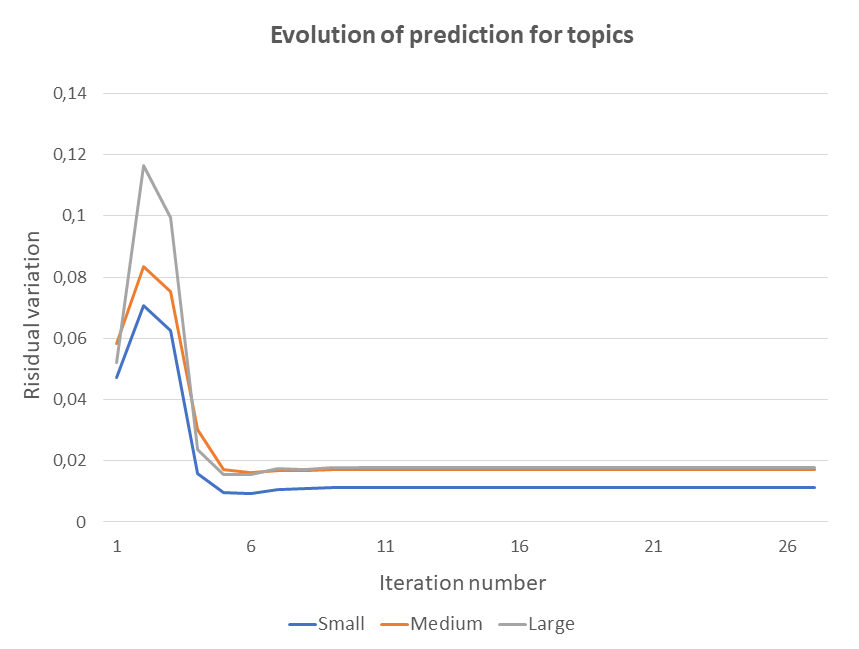
\includegraphics[width=0.75\linewidth]{Figures/chap5/total.png}}
		\caption{Variation résiduelle calculée entre la valeur de dominance réelle et celle prédite à chaque tour de dialogue} 
		\label{fig:converge}
	\end{figure}
	Nous avons également calculé le nombre moyen d'itérations afin de trouver la meilleure prédiction de $ dom_{other} $. Les résultats ont montré que l'agent a besoin de $4$ itérations en moyenne pour converger vers la meilleure prédiction des comportements de dominance.
	
	Nous avons étudié l'impact du nombre initial d'hypothèses $M_h$ sur la convergence de la prédiction. Nous avons voulu étudier si un grand nombre d'hypothèses nécessiterait des itérations supplémentaires pour converger. Par conséquent, nous avons comparé les résultats obtenus pour les conditions \emph {$\{$Petit, Medium, Large$\}$} sur la convergence de la négociation. Le graphique présenté dans la figure \ref {fig:converge} montre que notre algorithme converge rapidement, indépendamment de la taille du domaine de négociation. Nous pouvons observer que l'algorithme a pris deux itérations supplémentaires pour converger sur les domaines les plus larges par rapport aux domaines de taille moyenne et petite. La différence n'est pas significative pour affecter le comportement général de notre modèle.
	
	%	\begin{table}
	%		\
	%		\begin{tabular}{|p{3 cm}|c|c|c|}
	%			\hline
	%			Model size & Small & Medium & Large \\
	%			\hline
	%			Time execution (milliseconds) & 50.28 &	59.83 &	116.38\\
	%			\hline
	%		\end{tabular}
	%	\end{table}
	
	\subsubsection{Rapidité de raisonnement}
	Nous évaluons le temps d'exécution de l'algorithme afin d'étudier l'évolution du modèle de la théorie de l'esprit en fonction du complexité du domaine de négociation.
	
	Pour chaque dialogue, nous avons calculé le temps d'exécution moyen que met l'algorithme à faire une prédiction et ce à chaque tour de négociation. 
	Nous cherchons à étudier l'effet de la taille des hypothèses sur la rapidité de la prédiction à chaque tour. Les résultats sont présentés dans la figure \ref{fig:time}. En comparant  le temps d'exécution obtenu pour les domaines \emph{grand} et \emph{moyen}, nous observons que l'algorithme a pris en moyenne $12$ millisecondes de plus à chaque tour. Cependant, cette différence n'est pas significative puisque l'exécution totale reste très rapide.
	\begin{figure}[h]
		\fbox{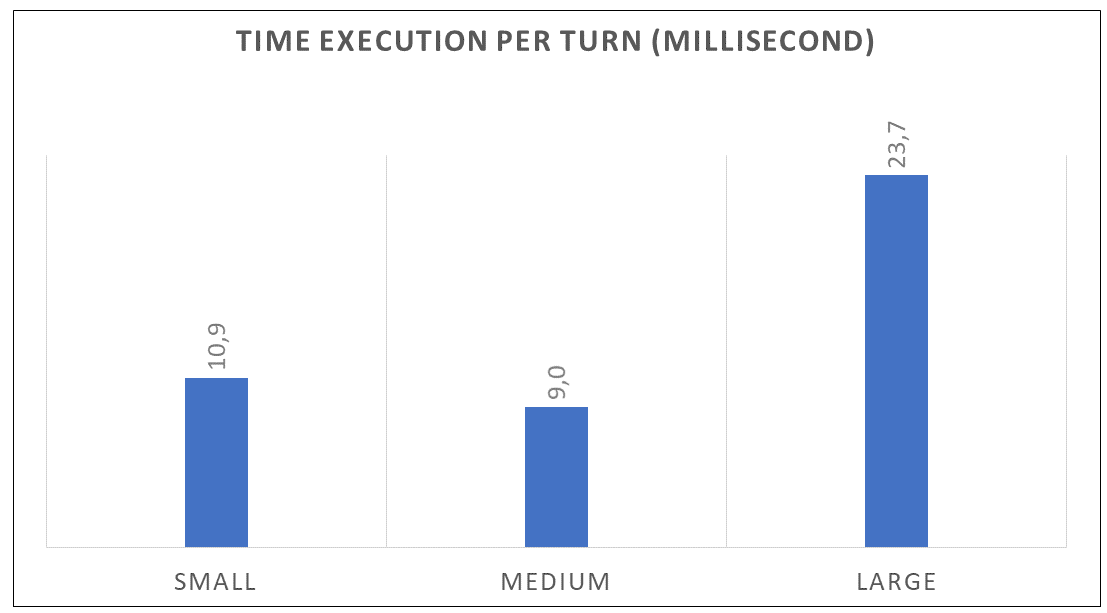
\includegraphics[width=\linewidth]{Figures/chap5/time_exec.png}}
		\caption{Le temps d'exécution de l'algorithme ToM à chaque tour de dialogue} 
		\label{fig:time}
	\end{figure}
	

	\subsection{Discussion}
	
	Nous avons analysé les performances de notre modèle de ToM tant sur l'aspect de la pertinence des prédictions que sur la rapidité d'exécution sur les différents domaines de négociation. Les résultats obtenus fournissent un support solide sur la précision du modèle de la ToM.
	 En effet, pour la plupart des dialogues générés, l'agent avec les capacités ToM était capable de prédire une approximation très proche du niveau de dominance de son interlocuteur. De plus, l'agent était capable de positionner l'interlocuteur sur le bon niveau de dominance qu'après deux tours de paroles et la meilleure évaluation après uniquement cinq tours. Ces comportements ont été générés dans un délai raisonnable, permettant à l'agent de produire des dialogues en temps réel.
	
	Ces résultats renforcent la précision de notre modèle et donnent de bonnes perspectives pour mettre en œuvre ce modèle dans le contexte de la négociation collaborative agent/humain. 
	
	Cependant, la validation présentée dans le contexte de la négociation agent/agent est une évaluation contrôlée puisque les deux agents utilisent le même modèle décisionnel. Cette situation augmente les chances de bonnes prédictions des comportements de dominance.
	Ainsi, notre modèle collaboratif de négociation doit être validé dans le contexte de la négociation humain/agent. Notre modèle initial présenté dans le chapitre \ref{chap:domer} repose sur des études de psychologie sociale. Il a été validé avec une étude perceptive où les participants humains étaient capables de percevoir et de reconnaître les comportements de dominance exprimés par les agents. Pour ces raisons, nous croyons que c'est une bonne approximation des comportements humains de dominance et nous attendons de bonnes prédictions de notre modèle ToM dans le contexte de négociations entre un agent et un humain.


\section{Conclusion}
	Ce chapitre a présenté un modèle de la ToM qui permet à l'agent d'utiliser des paradigmes de la théorie de l'esprit de simulation afin de prédire les comportements de dominance de son interlocuteur. Ce modèle est cruciale, car à travers ces prédictions, l'agent révise ses comportements de dominance dans le but de simuler une relation interpersonnelle de dominance avec son interlocuteur. 
	
	Ce modèle est une extension de notre modèle de négociation collaborative basé sur la dominance qui permet à l'agent d'utiliser son modèle décisionnel pour raisonner sur les comportements de dominance de son interlocuteur. Nous avons expliqué notre démarche pour utiliser les paradigmes de la \emph{théorie de simulation} afin d'implémenter le comportement de l'interlocuteur. 
	
	Le modèle proposé repose sur une représentation partielle de l'état mental de l'autre qui nous a poussé à adapter le processus décisionnel pour gérer les cas d'incertitudes. 
	
	Ce modèle a ensuite fait l'objet d'une évaluation agent/agent pour analyser la pertinence des prédictions de comportements de dominance. Les résultats obtenus montrent la justesses des prédictions fournis par le modèle de la ToM. Ces résultats sont encourageants, toutefois, une évaluation dans le contexte agent/humain où les comportements de l'utilisateur sont imprévisibles reste à faire. Le chapitre suivant s'attache donc à proposer une étude pour évaluer notre modèle de négociation collaborative dans le cadre une interaction agent/humain.
	
	